\documentclass[12pt]{report}
%\documentclass{article}
\usepackage[utf8]{inputenc}
\usepackage{graphicx}
\graphicspath{.}
\usepackage{fullpage}

\title{CSCE 315 \\ Initial Prototype}
\author{Oscar Reyes,\\
	James Corder Guy,\\
	Oleksandr Sofishchenko}
\date{April 18, 2017}

\begin{document}
	
	\maketitle
	
	\newpage
	
	\begin{center}
		\title{\textbf{Aggie Spirit Scheduling App}} \\
		
	\end{center}

	The goal of this project is to improve the user experience with the Texas A\&M bus route website and app. We aim to make a better interface for users and also to increase speed of the website. Currently, the official website http://transport.tamu.edu/busroutes/ has a minimalistic interface. This is something we would like to emulate but we wish to improve the quality of the application, make it look nicer. In addition, we want to increase the speed in which the website responds to requests once a button is pressed. \\
	
	We have a couple fall-back goals for our project. First we would like to track buses better. We would also like to show the location of the user in the map. We want to make the website more responsive on mobile. In addition, we want to show the things that are around the bus stops. Important places like grocery stores, apartments and other locations.\\
	
	In addition there are some reach goals. These are the goals that we would really like to have on the project if we have time for it. The first one is to show if a bus is early or late. We would also like to how much more time is left before a bus gets to its next stop. Furthermore, we would like to calculate how much time for a user to get to a selected bus stop. Finally, we would like to show traffic in our map.\\
	
	To get our project done we will be combining the Texas A\&M bus transportation data. It is in Json format and this is how we could get the information of the buses. In addition to that we will also be using the Google Maps API to be able to have a map in our website an to hopefully incorporate the tamu bus routes on top of it. Third, we will be using a responsive W3 framework from W3 schools, a website to learn HTML to have a template for our website.\\
	
	The reason we want to do this project is because we want users to have access to the bus route information faster than they do now. Our application would be ideal to help a freshman figure out where the bus stops are located in relation to him. It would also help a freshman know what key locations are around the bus routes. For example, a Walmart, HEB, a post office or maybe a mall. Another person that this could benefit would be students that are heading late to class. Sometimes alarm clocks are not enough to wake someone up or people forget to set them. Our application would help students leave on time from their place with the time estimate that it would take from their location to a selected stop and they could compare that to the estimated time for a bus to arrive to the bus stop that they are heading to. Finally, an improved tracking system will give all users in general a better idea of where buses currently are located because at the moment there is a delay to the update of bus locations.\\
	
	While we work on our project we will face a couple challenges. The first one will be connecting to the back-end to the client. Another problem we may face will be to connect the data pulled from transportation services and link it with the google maps API. The final trouble we might face will be to overlay things on top of the google maps application so we can show the routes properly. Furthermore, we will have to learn HTML 5 and CSS. We will also need to learn flask to parse the json data properly.\\
	
	The project will be organized in the following way. James Corder Guy is in charge of back-end development. Oleksandr Sofishchenko is in charge of front-end development. Oscar Reyes is in charge of project management, backlog and project submissions.\\
	
	The following sketches are mocks of what we would like our wbesite to look like. The first picture is the home page. It will have our team information, the university logo and an "Explore" button to go to the bus routes. This will all be on top of a maroon background. \\
	 
	 \begin{figure}[h]
	 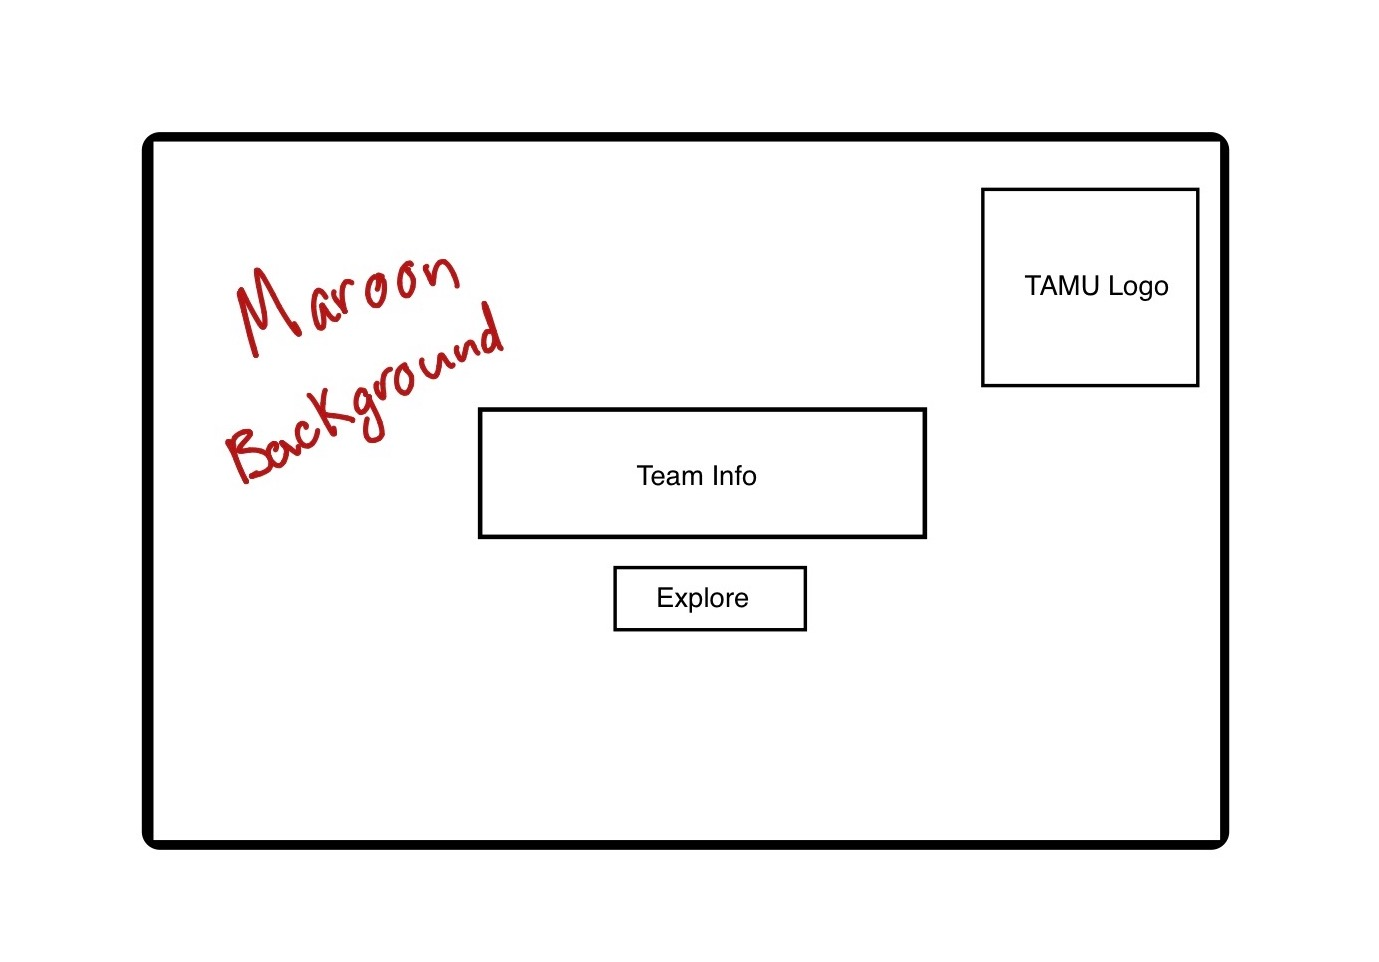
\includegraphics[scale=0.30]{Home}
	 \centering
     \end{figure}
 
 	\newpage
	
	Once the user clicks the "Explore" button it will take them to a screen where they can select their bus route. It should look something like the following.\\
	
	\begin{figure}[h]
		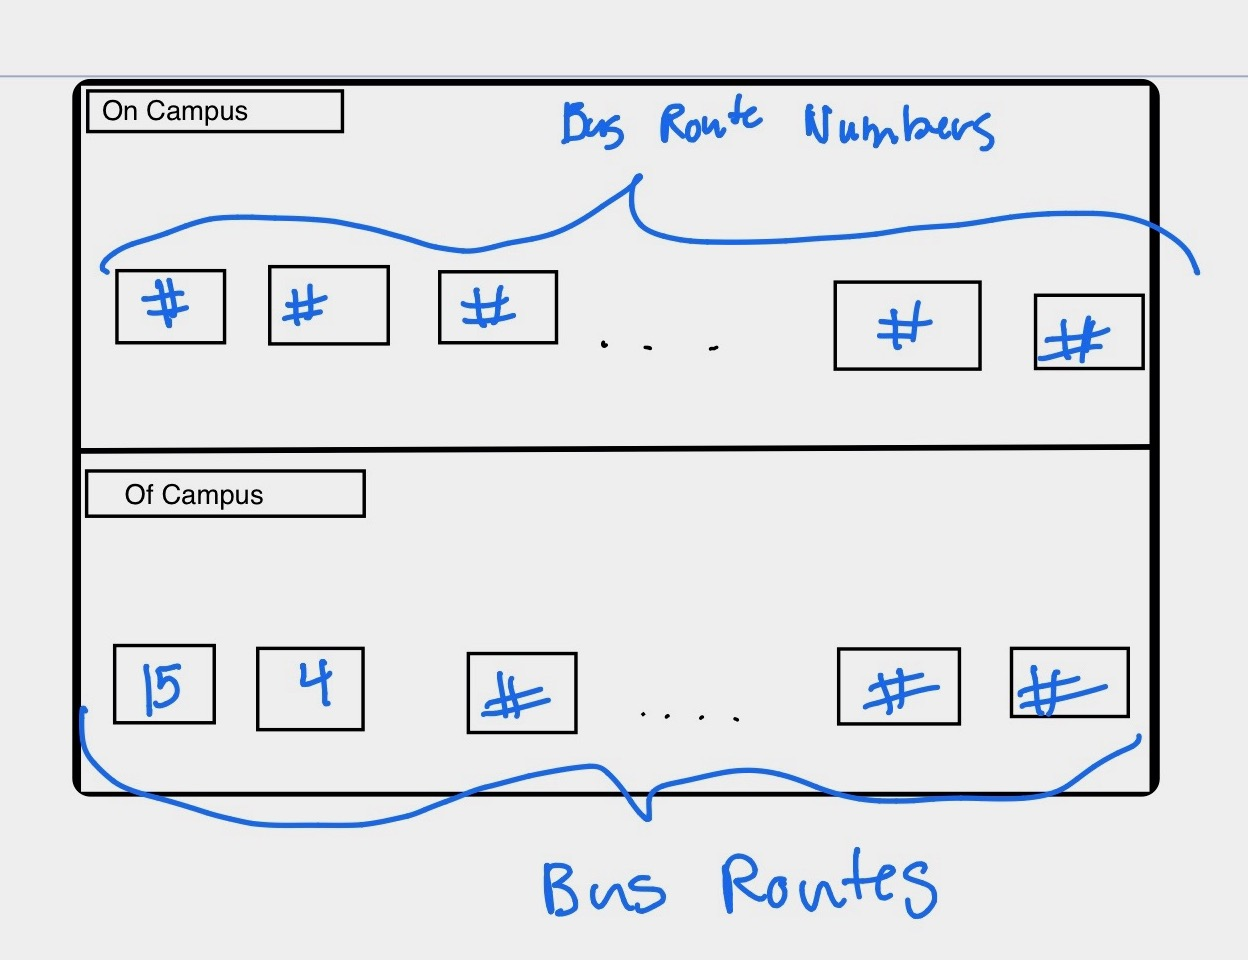
\includegraphics[scale=0.20]{BusRoutes}
		\centering
	\end{figure}
	
	Once the user selects the bus route, then the page will go to a map screen. There are two possible map screens. The first one is just a map.\\
	
	\begin{figure}[h]
		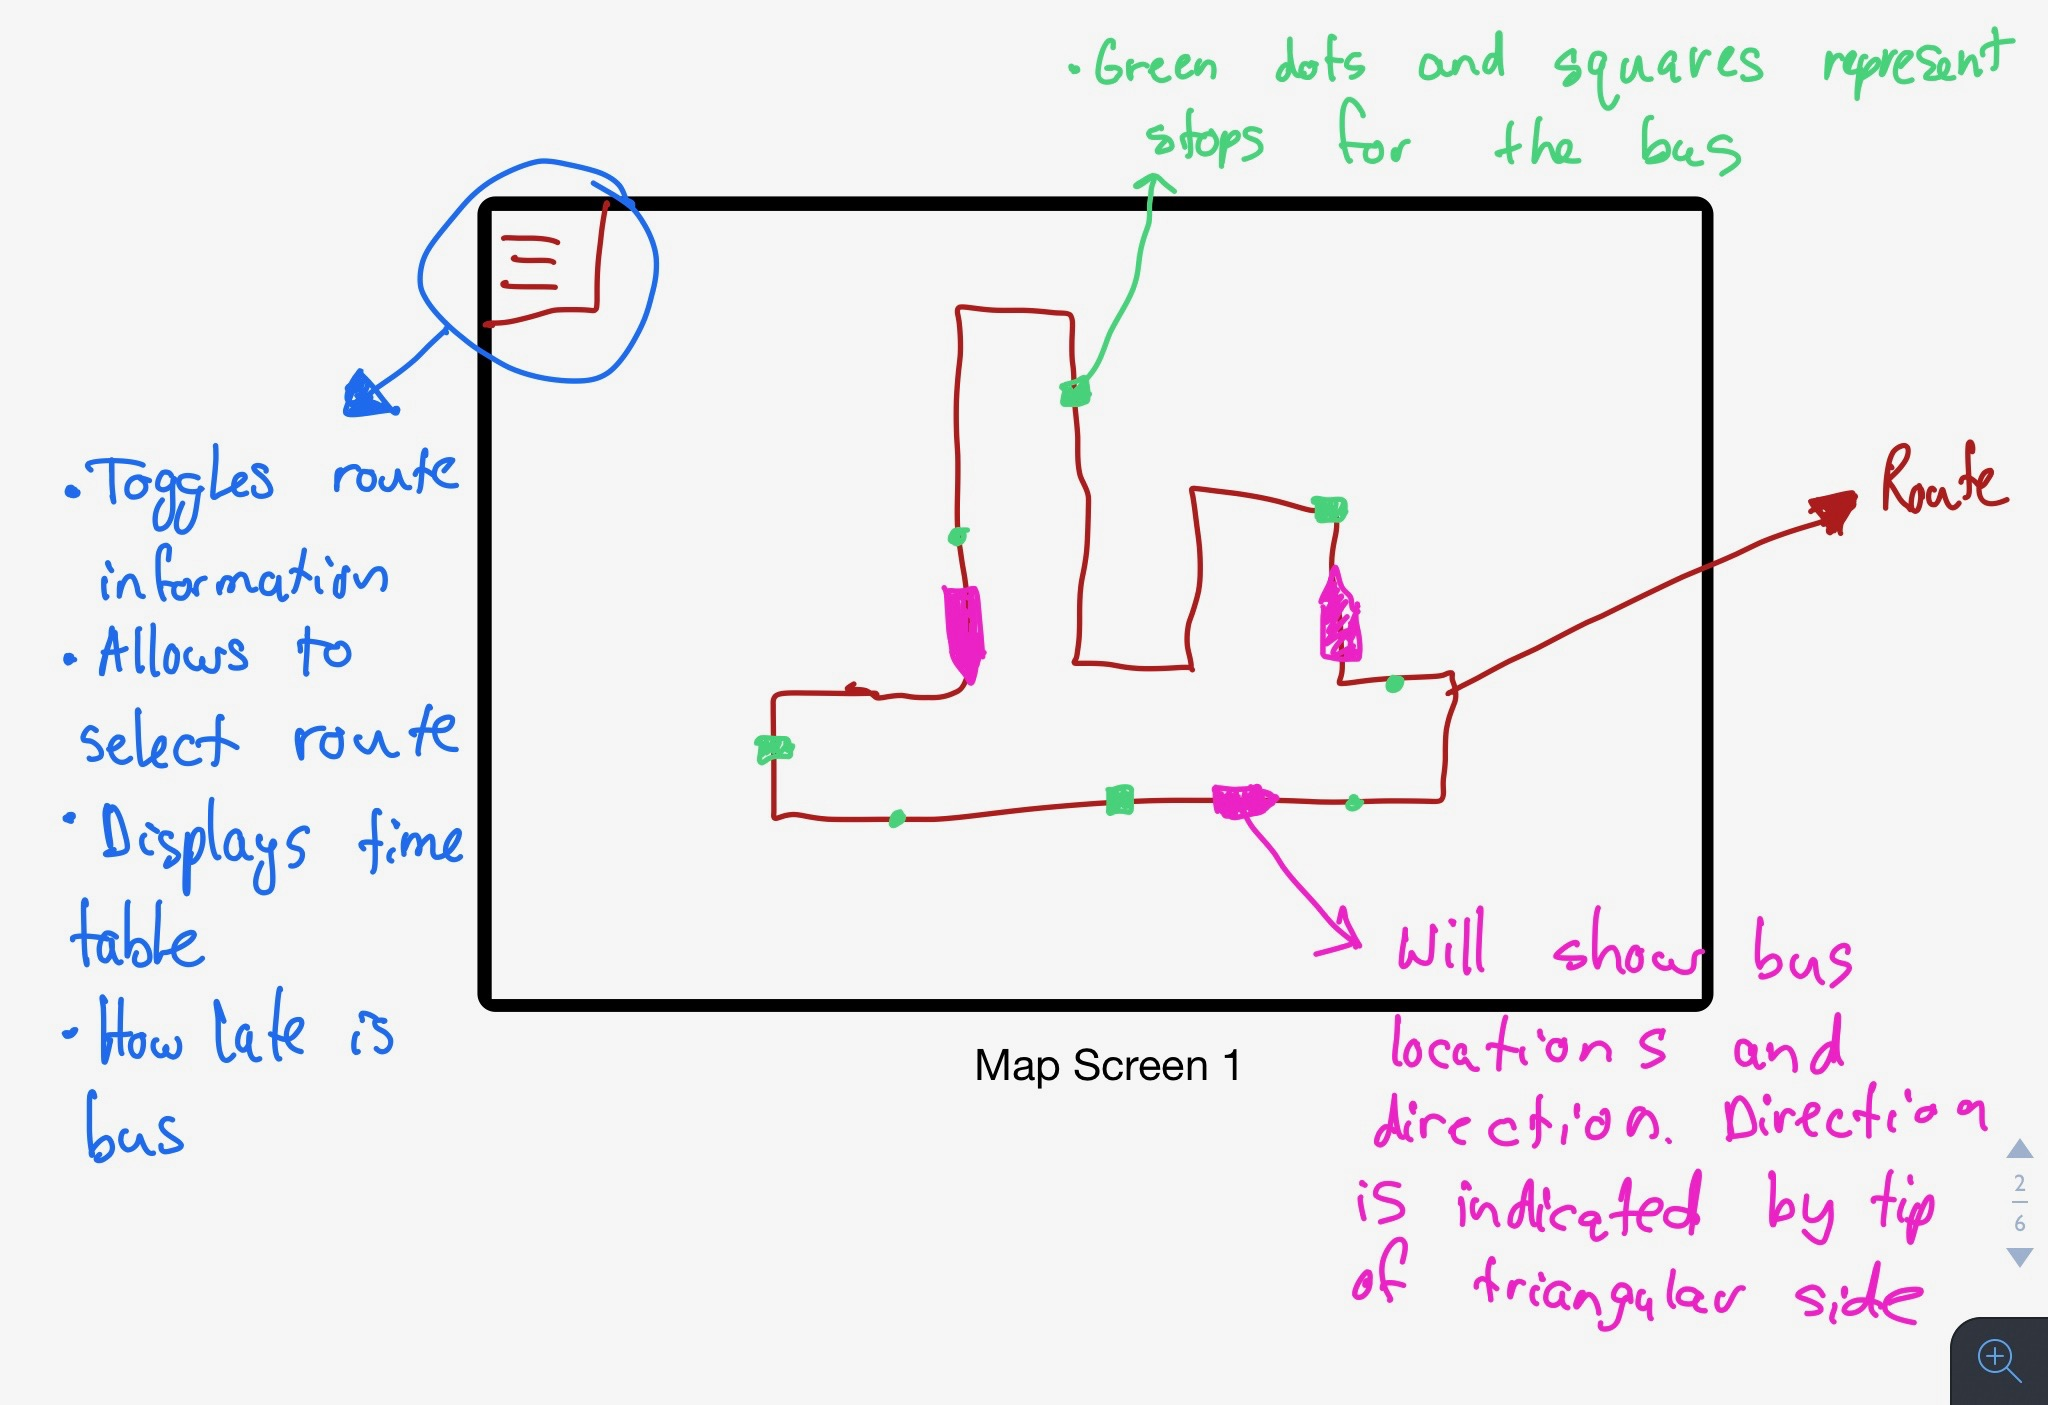
\includegraphics[scale=0.15]{MapScreen1}
		\centering
	\end{figure}
	\newpage
	
	On the first map screen, the user can then click the top left corner square to toggle more information on the bus routes. You will also be able to see the bus route schedule.\\
	
	\begin{figure}[h]
		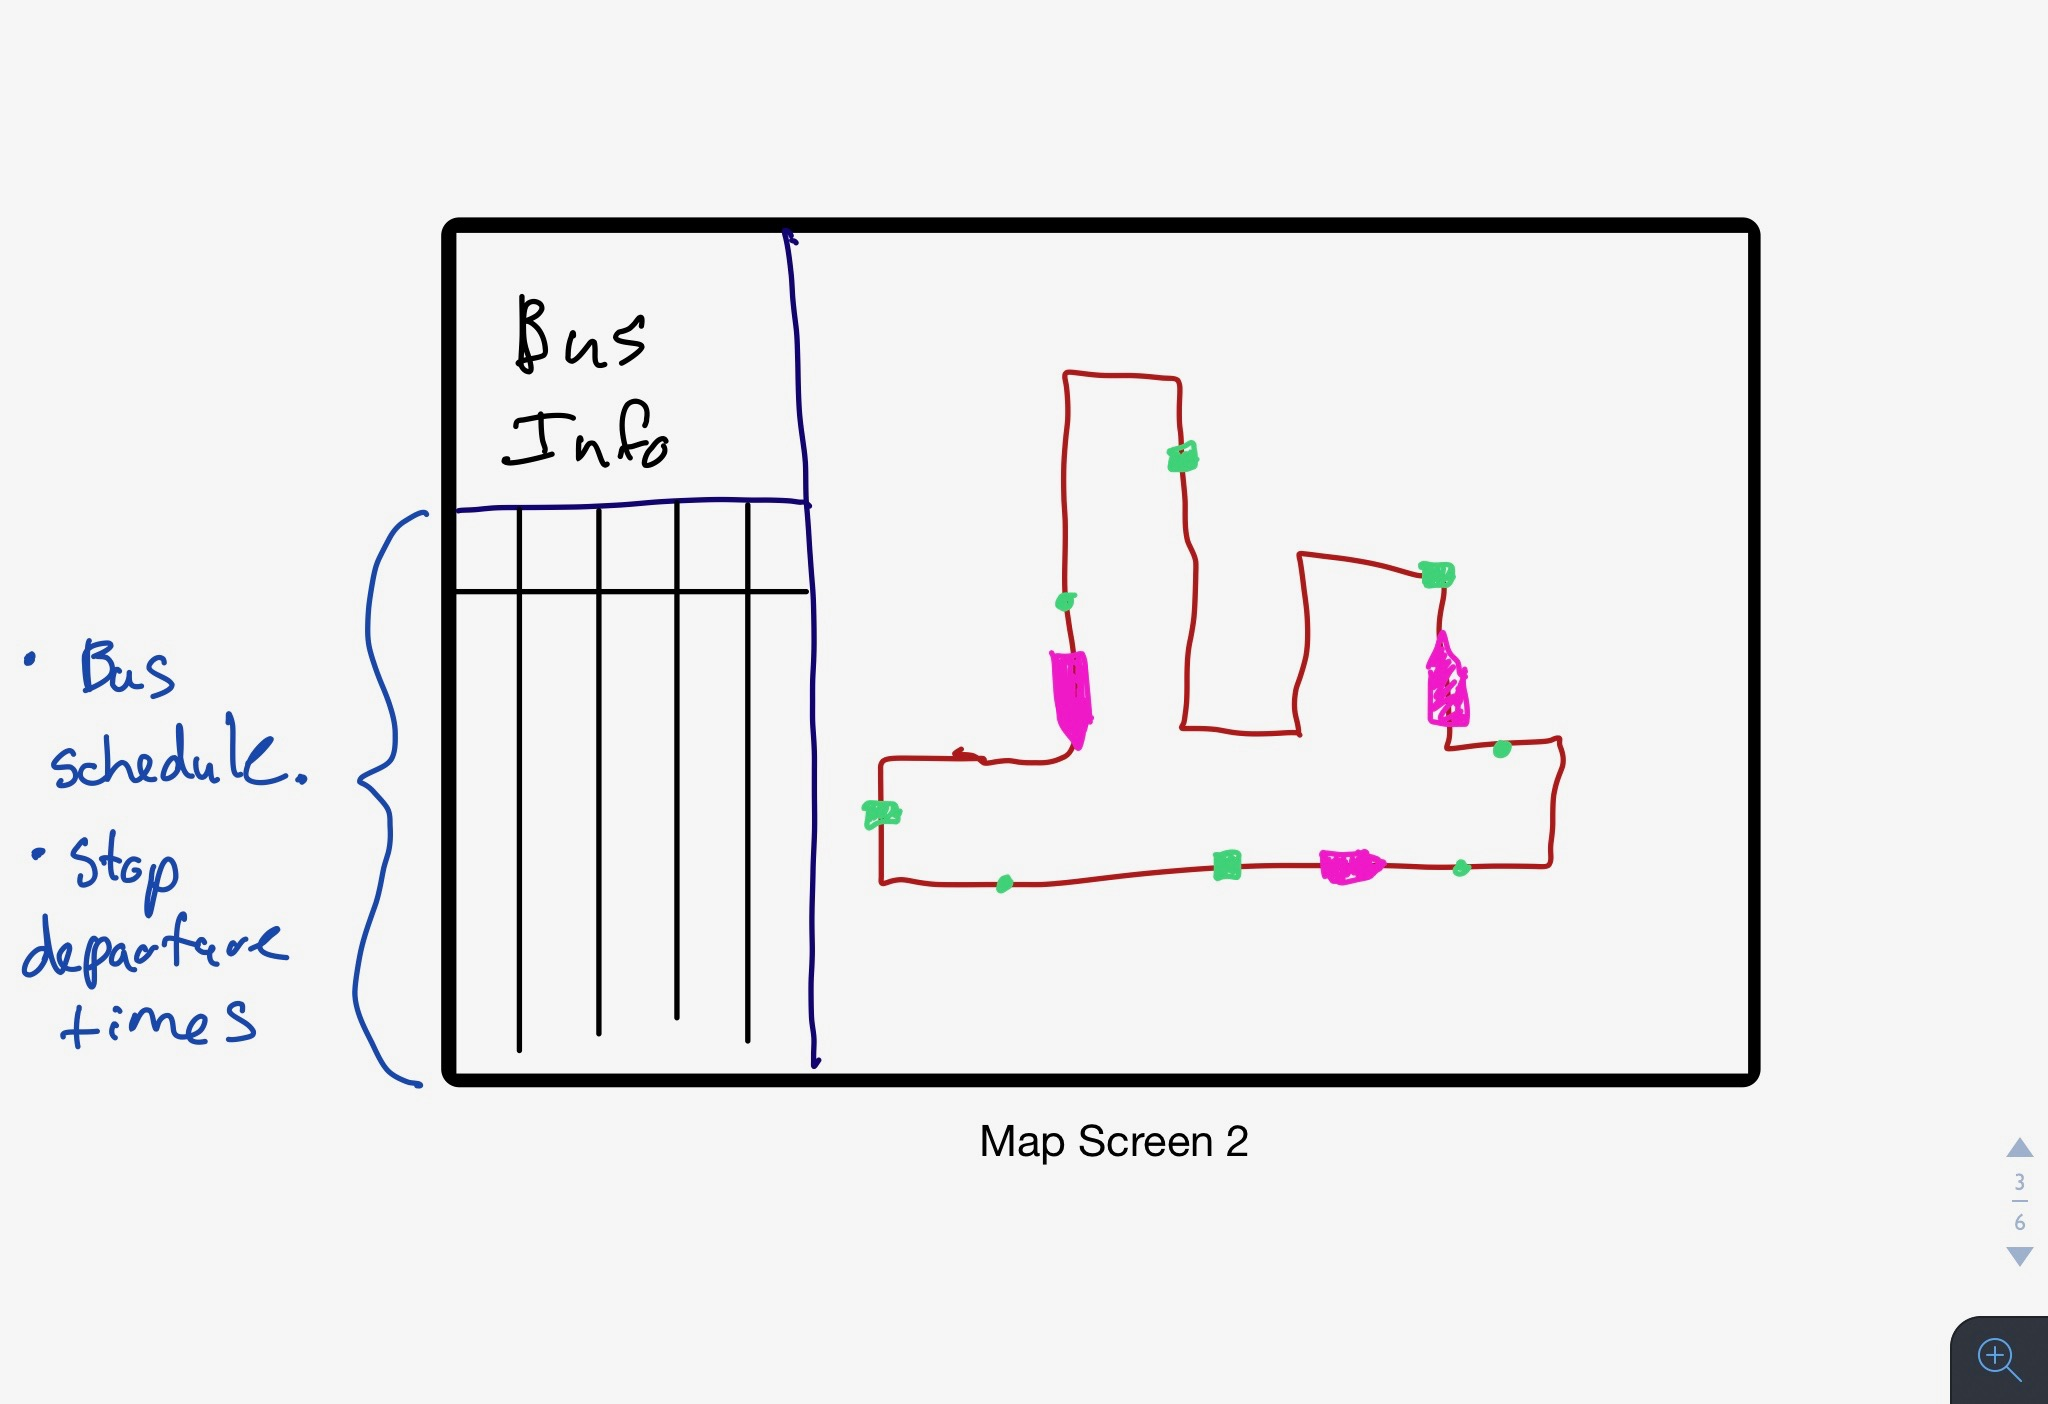
\includegraphics[scale=0.15]{MapScreen2}
		\centering
	\end{figure}
	
	
	Hopefully we will be able to have a functioning website with increased functionality so the user can have a better experience overall.
	
	
	
	
\end{document}